\documentclass[11pt]{beamer}

\usetheme{Madrid}
\usecolortheme{default}
\setbeamertemplate{navigation symbols}{}
\setbeamertemplate{footline}[frame number]

\usepackage[utf8]{inputenc}
\usepackage{graphicx}
\usepackage{listings}
\usepackage{xcolor}

\lstset{
  basicstyle=\ttfamily\small,
  breaklines=true,
  columns=fullflexible,
  backgroundcolor=\color{black!5},
  frame=single,
  framerule=0.3pt
}

\title{Neostat Document Intelligence}
\subtitle{Extraction, Validation, and API Platform for Financial Documents}
\author{Priyanshu}
\date{}

\begin{document}

\frame{\titlepage}

% ---------------------------------------------------------------
\section{Problem}
\begin{frame}{The Problem}
  \begin{itemize}
    \item Neostat needs structured, validated data out of scanned and photographed
      financial documents --- without a hand-built parser per document type.
    \item Two very different document families in the sample set:
      \begin{itemize}
        \item HDFC Bank annual report pages --- vector-drawn PDFs, \textbf{no text layer}
        \item Malaysian retail receipts --- photographed, skewed, dot-matrix print
      \end{itemize}
    \item The core risk of any LLM-based extraction pipeline: \textbf{silent
      hallucination} --- a wrong number that looks plausible. The system has to
      \emph{prove} it isn't doing that.
  \end{itemize}
\end{frame}

% ---------------------------------------------------------------
\section{Architecture}
\begin{frame}{Architecture}
  \begin{center}
    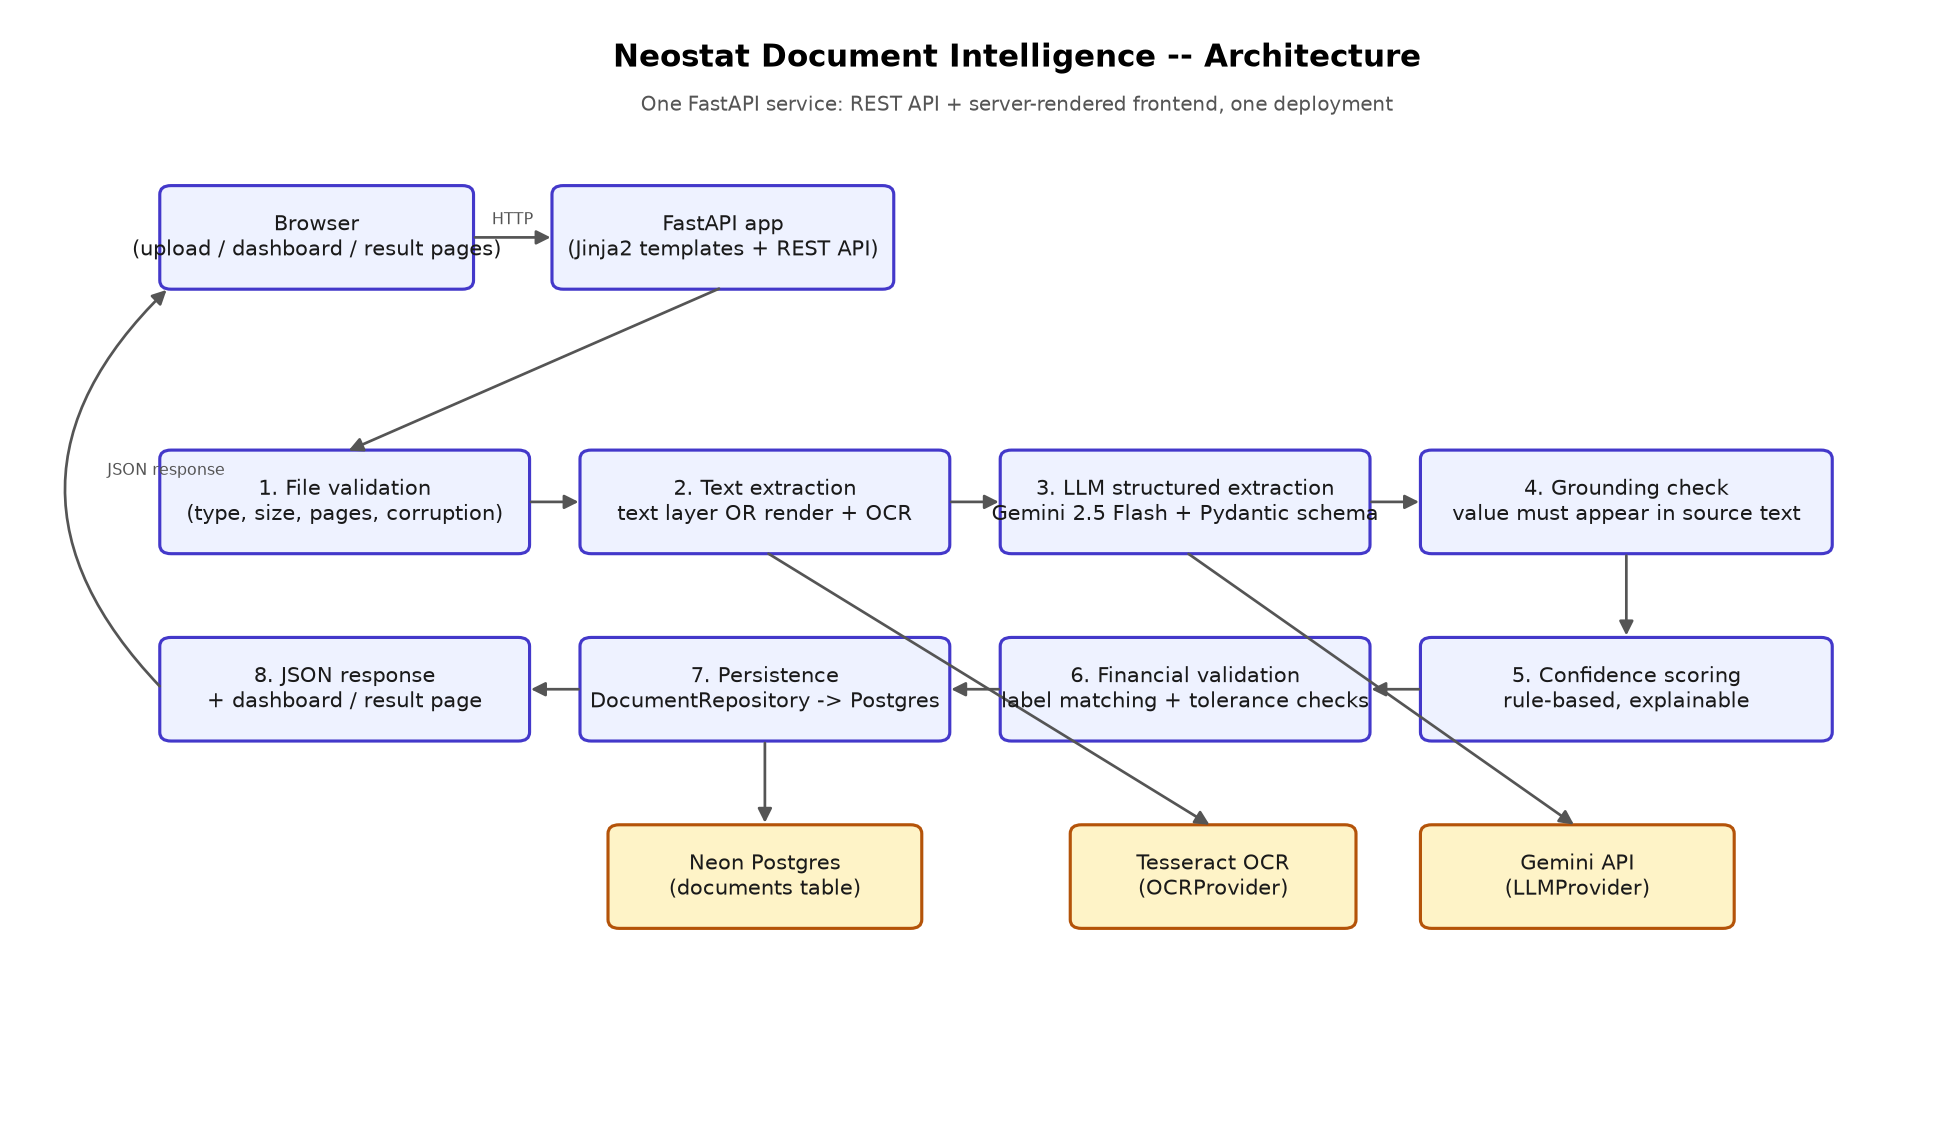
\includegraphics[width=0.95\textwidth]{architecture.png}
  \end{center}
\end{frame}

\begin{frame}{Architecture --- Key Decisions}
  \begin{itemize}
    \item One FastAPI service, one deployment: REST API + server-rendered frontend on
      the same origin.
    \item Eight-stage synchronous pipeline: validate $\rightarrow$ extract text
      $\rightarrow$ LLM structured extraction $\rightarrow$ ground $\rightarrow$
      score confidence $\rightarrow$ validate financials $\rightarrow$ persist
      $\rightarrow$ respond.
    \item Provider interfaces (\texttt{OCRProvider}, \texttt{LLMProvider}) so
      Tesseract/Gemini can be swapped without touching the pipeline.
  \end{itemize}
\end{frame}

% ---------------------------------------------------------------
\section{Pipeline Walkthrough}
\begin{frame}{Pipeline Walkthrough}
  \begin{itemize}
    \item \textbf{File validation:} sniffs the real content type from bytes (not the
      client's declared \texttt{Content-Type}), enforces size/page limits, rejects
      corrupted files --- before any paid API call.
    \item \textbf{Text extraction:} detect a usable PDF text layer ($>$100 chars) and
      use it directly; otherwise render the page at 300 DPI and OCR it with
      Tesseract.
    \item Most HDFC pages have no text layer at all, so render-then-OCR is the common
      path there; a few cash flow statements \emph{do} have a real text layer and
      take the faster, more accurate path.
  \end{itemize}
\end{frame}

\begin{frame}{One Real Example}
  \begin{itemize}
    \item Rendered page image $\rightarrow$ OCR text $\rightarrow$ final extracted
      JSON, side by side.
    \item Example: a Malaysian receipt (\texttt{FUYI MINI MARKET}) --- shop name,
      registration number, GST ID, line item, and both the inclusive-GST total and
      the cash/change all extracted correctly and verified against the source image
      by hand.
  \end{itemize}
\end{frame}

% ---------------------------------------------------------------
\section{Extraction Approach}
\begin{frame}{Extraction Approach and Prompt Design}
  \begin{itemize}
    \item One Pydantic schema per document type. Financial statements carry
      \texttt{periods} + \texttt{line\_items[].values} as a list of
      \texttt{\{period, value\}} pairs, preserving comparative columns instead of
      flattening them.
    \item The LLM gets: document type, the page image, OCR text with line numbers,
      and the target JSON schema (Gemini's structured-output mode).
  \end{itemize}
\end{frame}

\begin{frame}{Prompt Rules}
  \begin{itemize}
    \item Transcribe \emph{every} visible line item --- not a fixed list.
    \item Return \texttt{null} for anything unreadable, never guess.
    \item Preserve label text verbatim.
    \item Convert bracketed negatives to negative numbers, e.g.\
      \texttt{(1,546.40)} $\rightarrow$ \texttt{-1546.40}.
    \item Quote the exact source line for every field in \texttt{source\_text}.
    \item A schema validation failure triggers exactly one retry with the error
      appended to the prompt.
  \end{itemize}
\end{frame}

% ---------------------------------------------------------------
\section{Grounding and Confidence}
\begin{frame}{Grounding: Catching Hallucination}
  \begin{itemize}
    \item After extraction, every numeric value is checked against the page's source
      text (comma / bracket / currency-normalized).
    \item A value that isn't found is flagged \texttt{grounded: false} and its
      confidence drops sharply.
    \item This is the concrete answer to: \emph{``how do you know it didn't just
      make that up?''}
  \end{itemize}
\end{frame}

\begin{frame}{Confidence Formula}
  \[
    \text{confidence} = \text{source\_confidence} \times \text{grounding\_multiplier}
    \times \text{validation\_penalty}
  \]
  \begin{itemize}
    \item \textbf{source\_confidence:} 0.99 for a native text layer, else the
      Tesseract word confidence for the matched OCR token.
    \item \textbf{grounding\_multiplier:} 1.0 if grounded, 0.35 if not found in the
      source text at all.
    \item \textbf{validation\_penalty:} 0.85 if the field is an operand in a
      \emph{failing} financial check.
    \item Fully rule-based, documented in the README, \textbf{never} LLM-generated.
  \end{itemize}
\end{frame}

\begin{frame}{An Honest Limitation}
  \begin{itemize}
    \item Real example: OCR occasionally splits a large number across two tokens
      because of a stray rendering space.
    \item The value is actually correct, but strict text-matching flags it
      \texttt{grounded: false}.
    \item Left as a documented tradeoff --- ``fixing'' it by merging adjacent tokens
      risks merging two genuinely separate numbers instead.
  \end{itemize}
\end{frame}

% ---------------------------------------------------------------
\section{Financial Validation}
\begin{frame}{Financial Validation}
  \begin{itemize}
    \item Every check: \texttt{PASS} / \texttt{FAIL} / \texttt{NOT\_APPLICABLE}.
    \item \texttt{NOT\_APPLICABLE} whenever an operand is missing --- never
      substitute a zero.
    \item Line items matched to formula operands by \textbf{normalized label + a
      synonym map}, not row position.
    \item Tolerance: $|\text{variance}| \le \max(\text{ABS\_TOL},\ \text{REL\_TOL}
      \times |\text{reported}|)$, configurable via env.
    \item Checks run once per comparative period (HDFC pages show two years side by
      side).
  \end{itemize}
\end{frame}

\begin{frame}{Example Checks}
  \begin{itemize}
    \item \textbf{Invoice:} \texttt{quantity * unit\_price} $\approx$ line total;
      inclusive- and exclusive-GST total checks; \texttt{cash - total} $\approx$
      \texttt{change}.
    \item \textbf{Balance sheet:} \texttt{total\_capital\_and\_liabilities} $\approx$
      \texttt{total\_assets}; component sums per section.
    \item \textbf{P\&L:} income and expenditure chains down to net profit
      attributable to the group.
    \item \textbf{Cash flow:} operating + investing + financing + FX $\approx$ net
      increase in cash; opening + net increase $\approx$ closing cash.
  \end{itemize}
\end{frame}

% ---------------------------------------------------------------
\section{API and Demo}
\begin{frame}[fragile]{API}
  \begin{itemize}
    \item Live Swagger docs at \texttt{/docs}.
  \end{itemize}
  \begin{lstlisting}
curl -X POST https://<host>/api/v1/documents/process \
  -F "file=@invoice.jpg" -F "document_type=invoice"

curl https://<host>/api/v1/documents/invoice.jpg

curl https://<host>/api/v1/documents?limit=20
  \end{lstlisting}
\end{frame}

\begin{frame}{Demo}
  \begin{itemize}
    \item Upload page $\rightarrow$ processing $\rightarrow$ result page.
    \item Result page highlights: missing values, failed checks, low confidence, and
      ungrounded values --- with a legend.
    \item Dashboard: search and filter across all processed documents.
  \end{itemize}
\end{frame}

% ---------------------------------------------------------------
\section{Engineering Practices}
\begin{frame}{Engineering Practices}
  \begin{itemize}
    \item Structured JSON logging with a request ID on every line, one line per
      pipeline stage.
    \item A typed \texttt{AppError} hierarchy mapped to mandated error codes; a
      catch-all handler ensures no stack trace or secret ever reaches the client.
    \item All database access goes through one repository class --- routes never
      touch a session directly.
    \item 59 tests, run without network access or an API key (LLM and OCR providers
      are mocked).
  \end{itemize}
\end{frame}

% ---------------------------------------------------------------
\section{Results}
\begin{frame}{Results on the Sample Set}
  \begin{itemize}
    \item All 10 HDFC balance sheets (2017--2026) processed against the
      \textbf{real} Gemini API --- every one passed every financial check on both
      comparative years, confidence ranging 0.60--0.94.
    \item One cash flow statement and one invoice also passed for real, all checks
      green.
    \item The free-tier key's 20-requests/day cap was hit partway through the full
      50-document batch --- re-running the batch script once quota resets fills in
      the rest without reprocessing what already succeeded.
  \end{itemize}
\end{frame}

% ---------------------------------------------------------------
\section{Limitations and Roadmap}
\begin{frame}{Known Limitations}
  \begin{itemize}
    \item Grounding is a strict text match --- OCR token-splitting can flag a correct
      value as ungrounded.
    \item Validation-failure confidence penalty currently applies to invoice fields
      only, not financial-statement line items.
    \item No background job queue --- large batches would need one.
    \item Section matching (assets vs.\ liabilities) relies on the LLM populating a
      consistent \texttt{section} label.
  \end{itemize}
\end{frame}

\begin{frame}{Production Roadmap}
  \begin{itemize}
    \item Async processing with a job queue and status polling.
    \item A second OCR/LLM provider as an automatic fallback under rate limiting.
    \item Extend the validation-failure confidence penalty to financial-statement
      line items.
    \item Per-document-type prompt tuning based on measured accuracy against a
      larger labeled sample.
    \item Authentication on the API.
  \end{itemize}
\end{frame}

% ---------------------------------------------------------------
\begin{frame}
  \centering
  \Large Thank you
  \vspace{1em}

  \normalsize
  \url{https://github.com/deathKiller10/neostat}
\end{frame}

\end{document}
